\documentclass[conference]{IEEEtran}
\usepackage{amsmath}
\usepackage{graphicx}
\usepackage{booktabs}
\usepackage{cite}
\usepackage{hyperref}

\setlength{\textfloatsep}{5pt plus 1pt minus 1pt}
\setlength{\dbltextfloatsep}{5pt plus 1pt minus 1pt}
\setlength{\abovecaptionskip}{2pt}
\setlength{\belowcaptionskip}{1pt}
\renewcommand{\dbltopfraction}{0.92}
\setcounter{dbltopnumber}{2}

\title{Microresonance: Wireless 802.11 TSF-Coherent Active Acoustic Probing of the Skeletal Waveguide for Real-Time Isometric Motor Intent and Posture Decoupling}

\author{
\IEEEauthorblockN{Amir Fatkulin}
\IEEEauthorblockA{Independent Research, Kyiv, Ukraine\\
Patent: WO/2026/229867 (PCT/IB2026/054169) \quad $|$ \quad Zenodo DOI: \href{https://doi.org/10.5281/zenodo.24533996}{10.5281/zenodo.24533996}\\
Code \& Raw Data: \url{https://github.com/itsme228/microresonance}}
}

\begin{document}
\maketitle

\begin{abstract}
Non-invasive extraction of voluntary motor intent via surface electromyography (sEMG) suffers from skin-electrode impedance drift, sweat degradation, inability to operate through clothing, and severe baseline saturation under orthostatic load. Recent wearable vibroacoustic systems such as WAVES (Nov.~2026) estimate passive resting muscle stiffness via wired multi-IMU arrays and pulsed soft-tissue Time-Difference-of-Arrival (TDoA) over $2.5\text{--}8.5\text{ cm}$, requiring bare-skin adhesives and $1\text{--}2\text{ min}$ per reading. We present \textit{Microresonance}, a dry, through-clothing wireless neuromuscular interface ($<\$100$ prototype BOM) that treats the limb as a \textit{low-loss skeletal waveguide (bone) shunt-loaded by tunable viscoelastic muscle--tendon resonators} - analogous to damping a guitar string. Two untethered ESP32-S3 nodes - a lumbar waist emitter belt and a distal ankle (lateral malleolus) 20-bit ADXL355 receiver strap ($\sim 0.9\text{ m}$ skeletal path) - achieve sub-2~$\mu$s wireless clock coherency via hardware IEEE 802.11 TSF timestamps, yielding a $3.01^\circ$ ($0.05\text{ rad}$) resting phase noise floor at $33.4\text{ Hz}$ ($30\text{ ms}$ latency) and $99.9\%$ lock stability. In a single-subject ($N=1$) multi-posture proof-of-concept ($5\text{ s}$ lower-limb isometric cycles across seated, leg-extended, and standing orthostatic regimes; $5{,}136$ frames), $500\text{ Hz}$ acoustic phase achieves $28.2\text{--}33.0\text{ dB}$ non-circular protocol-frequency SNR ($0.10\text{ Hz}$), outperforming concurrent sEMG by $18.1\text{--}26.7\text{ dB}$ and IMU tilt by $9.8\text{--}12.4\text{ dB}$. While standing elevates the sEMG floor $20.7\times$, acoustic phase preserves discrete isometric steps ($66.1^\circ$, Cohen's $d=3.57$). In this $N=1$ evaluation, inter-axis polarization $(\Delta\phi_{XY},\Delta\phi_{YZ})$ yields $100.0\%$ IMU-free posture accuracy and $92.8\%$ 6-state chronological holdout accuracy (Silhouette $+0.46$ vs.\ $-0.24$ for sEMG), while phase velocity $|d\phi/dt|$ tracks gyroscope macro-motion ($r=0.59$) with $17.9\times$ separation for IMU-free motion self-gating.
\end{abstract}

\begin{IEEEkeywords}
Active acoustic sensing, skeletal waveguide, lock-in amplifier, IEEE 802.11 TSF, neuromuscular interface, ESP32-S3.
\end{IEEEkeywords}

\section{Introduction}
\begin{figure*}[!t]
\centering
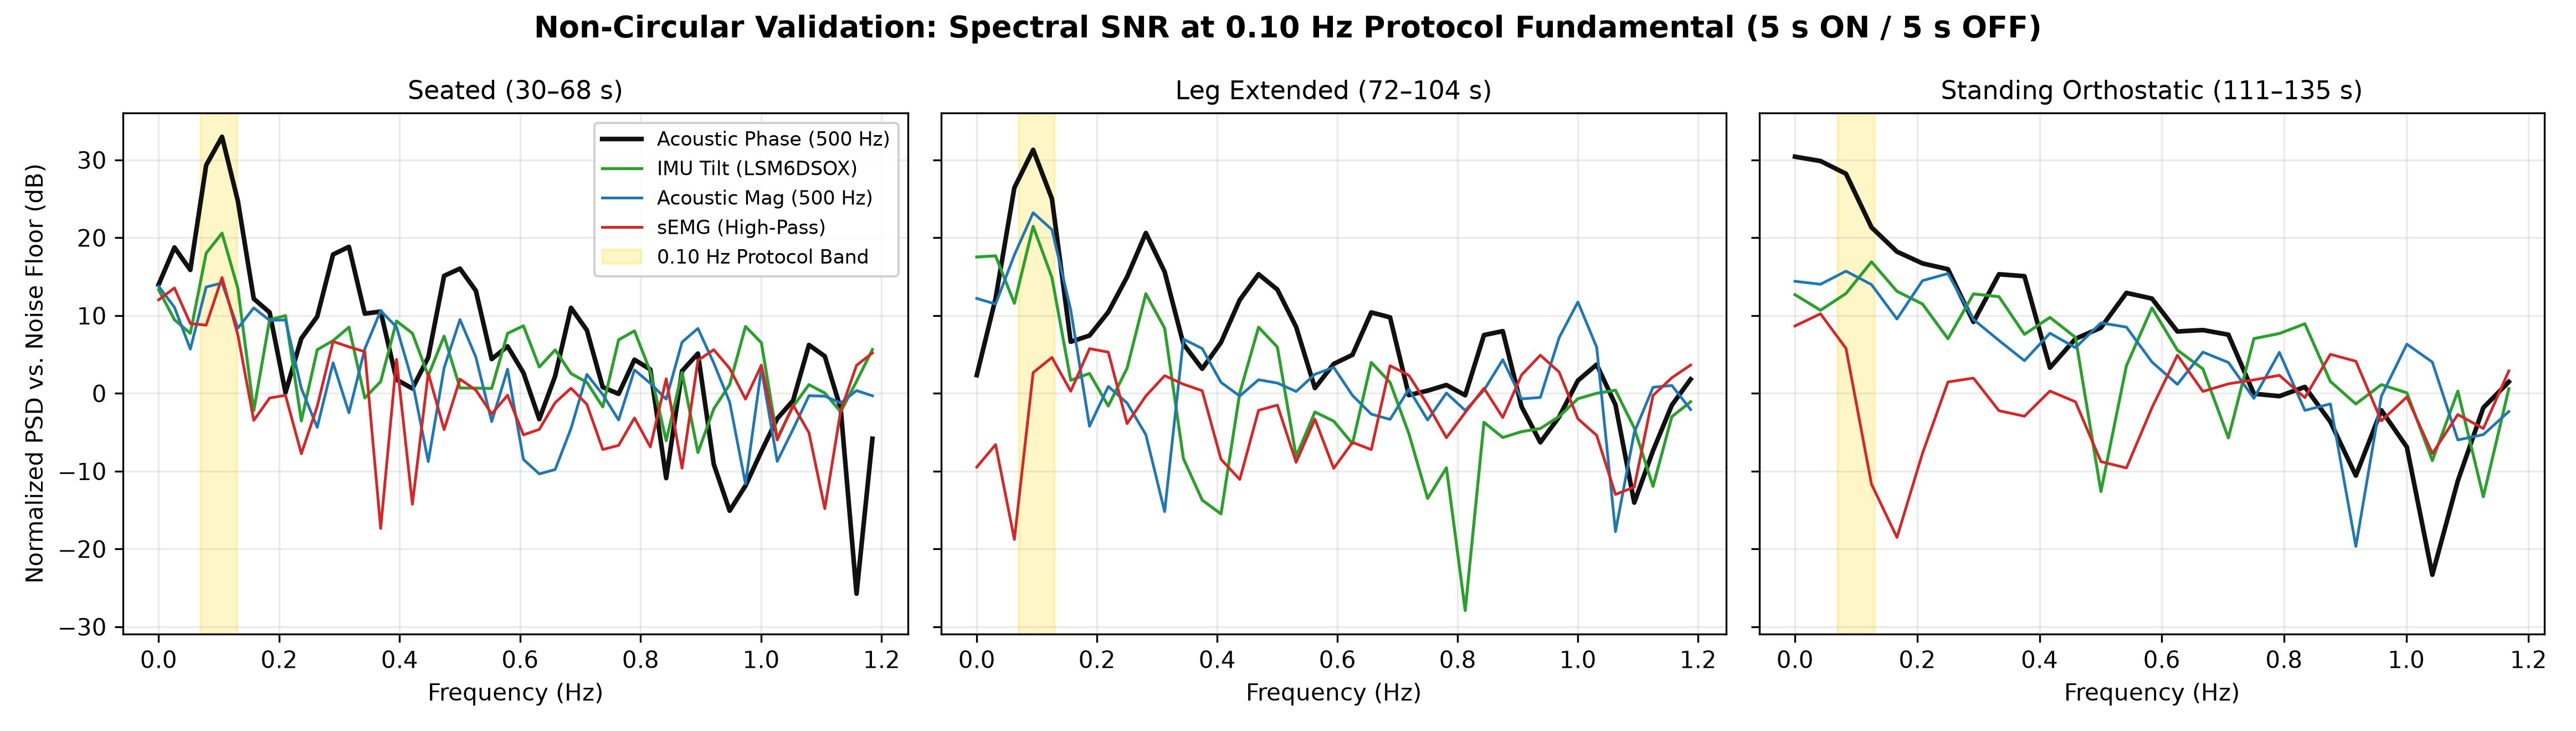
\includegraphics[height=1.24in]{figures/fig2_noncircular_snr_spectra.png}
\caption{Non-circular spectral validation at the $0.10\text{ Hz}$ protocol fundamental ($5\text{ s}$ ON / $5\text{ s}$ OFF) across seated, leg-extended, and standing orthostatic regimes. Coherent $500\text{ Hz}$ acoustic phase outperforms high-pass sEMG ($+18.1\text{ to }+26.7\text{ dB}$) and co-located IMU tilt ($+9.8\text{ to }+12.4\text{ dB}$).}
\label{fig:snr}
\end{figure*}
Wearable human-computer interaction (AR/VR neural wristbands), bionic prosthetics, and assistive exoskeletons require reliable, low-latency detection of voluntary isometric motor intent under everyday conditions. Surface electromyography (sEMG) remains the incumbent modality, yet microvolt-scale biopotentials demand bare-skin contact and degrade sharply with sweat, electrode lift-off, and postural recruitment - standing induces continuous orthostatic tetanus that masks discrete voluntary contractions. Passive mechanomyography (MMG) and bio-acoustic sensing~\cite{laput2016viband} operate dry, but low-frequency bands ($5\text{--}40\text{ Hz}$) overlap directly with limb motion. Ultrasound sonomyography (SMG)~\cite{akhlaghi2016smg} and shear-wave elastography~\cite{gennisson2013elastography} observe tissue mechanics directly, but require acoustic gel, piezo arrays, and bulky high-voltage electronics.

Active vibroacoustic probing bridges this gap by injecting controlled mechanical excitations into the limb. Recently, Rohal \textit{et al.} introduced \textit{WAVES}~\cite{rohal2026waves}, using an ESP32-S3, bone-conduction exciter, and wired array of three IMUs to estimate passive resting muscle stiffness via pulsed soft-tissue TDoA over $2.5\text{--}8.5\text{ cm}$. However, WAVES targets passive resting stiffness rather than voluntary motor intent: its pulsed TDoA pipeline rejects $33\text{--}98\%$ of on-body trials, requires $50\text{--}100$ pulses ($1\text{--}2\text{ min}$) per reading, degrades at high stiffness as $\Delta t$ shrinks, and requires bare-skin adhesives aligned with a 3D-printed stencil because straps or clothing corrupt envelope arrival times.

\textit{Microresonance} takes a fundamentally different physical and architectural approach: instead of tracking short-range soft-tissue shear pulses, it injects a continuous $500\text{ Hz}$ carrier into the \textit{skeletal waveguide (cortical bone)} and measures how surrounding muscles and tendons modulate the waveguide's complex transfer function via \textit{wireless 802.11 TSF-coherent I/Q lock-in demodulation}~\cite{ieee80211}:
\begin{enumerate}
    \item \textbf{Zero-Wire Sub-2~$\mu$s Phase Coherency:} Two independent ESP32-S3 nodes (waist belt to ankle strap, $\sim 0.9\text{ m}$) lock to hardware 802.11 TSF clocks, eliminating cables and crystal drift.
    \item \textbf{Real-Time ($30\text{ ms}$) Through-Clothing Isometric Intent:} A single 20-bit ADXL355 isolates $2\text{--}3\text{ mg}$ carrier phasors at $33.4\text{ Hz}$ through clothing ($28.2\text{--}33.0\text{ dB}$ non-circular SNR; $+18.1\text{ to }+26.7\text{ dB}$ over sEMG, $+9.8\text{ to }+12.4\text{ dB}$ over IMU tilt).
    \item \textbf{State-Space Islands \& Posture Orthogonalization:} Inter-axis polarization $(\Delta\phi_{XY}, \Delta\phi_{YZ})$ classifies three postures at $100\%$ accuracy without an IMU, and combined with $(\phi_Z, M_Z)$ resolves six biomechanical states at $92.8\%$ holdout accuracy ($N=1$).
    \item \textbf{IMU-Free Motion Self-Gating via $|d\phi/dt|$:} Acoustic phase velocity mirrors a gyroscope ($r = 0.59$) with $17.9\times$ separation between posture transitions and isometric onsets.
\end{enumerate}

\section{Physical Principle and System Architecture}

\subsection{Skeletal Waveguide with Muscle-Impedance Loading}
In our experimental geometry, the active $500\text{ Hz}$ emitter is worn on the lumbar waist belt while the receiver strap is placed distally above the ankle (lateral malleolus) - a $\sim 0.8\text{--}1.0\text{ m}$ path spanning the pelvis, femur, knee joint, and tibia/fibula. At $500\text{ Hz}$, soft-tissue shear waves attenuate within centimeters, whereas cortical bone conducts mechanical waves across the entire limb with low loss. We therefore model the limb as a \textit{skeletal waveguide (bone) shunt-loaded by tunable viscoelastic resonators (muscles and tendons)} - building on the biomechanical ``muscle tuning'' paradigm~\cite{nigg2001tuning,wakeling2001leg} and analogous to damping a guitar string. Letting $Z_0 > 0$ denote the bone waveguide characteristic impedance and $Z_m(\omega; G, \eta) = R_m(\eta) + jX_m$ with $X_m = \omega m_{\text{eff}} - k(G)/\omega$ the coupled muscle--tendon load, the transfer function $H(\omega)$ and phase shift $\Delta\phi$ follow:
\begin{equation}
H(\omega) = \frac{H_0(\omega)}{1 + \alpha\, Z_m(\omega; G, \eta)/Z_0}, \quad \Delta\phi = \arg\!\frac{H_{\text{contracted}}(\omega)}{H_{\text{relaxed}}(\omega)}.
\end{equation}
With real $Z_0 > 0$ and $\alpha > 0$, $\arg H = \arg H_0 - \arctan(\alpha X_m / (Z_0 + \alpha R_m))$, so $\partial(\arg H)/\partial k$ keeps a single sign across $\omega$ (phase-sign inversion requires concurrent shifts in $m_{\text{eff}}$ or $R_m$). Instead, Eq.~(1) predicts a falsifiable \textit{amplitude-sign inversion across resonance $\omega_0 = \sqrt{k/m_{\text{eff}}}$}: above $\omega_0$ ($X_m > 0$), increasing $k$ reduces $|X_m|$ and raises $|H|$ - matching our $+11\text{--}16\%$ gain at $500\text{ Hz}$ (above typical tens-of-Hz leg soft-tissue resonances~\cite{wakeling2001leg}) - whereas below $\omega_0$ ($X_m < 0$), contraction must attenuate $|H|$. This model is consistent with: (i) $2\text{--}3\text{ mg}$ survival over $\sim 0.9\text{ m}$, (ii) bounded phase leads ($\Delta(\arg H) = +36^\circ\text{ to }+67^\circ$, observed as a drop in demodulated lag $\phi$) paired with $|H|\uparrow$ ($+11\text{--}16\%$) at $500\text{ Hz}$ under stiffness increase $k\uparrow$, and (iii) sharp 3D polarization shifts ($\Delta\phi_{XY}, \Delta\phi_{YZ}$) when hip/knee angles alter bone-segment coupling.

\begin{figure}[t]
\centering
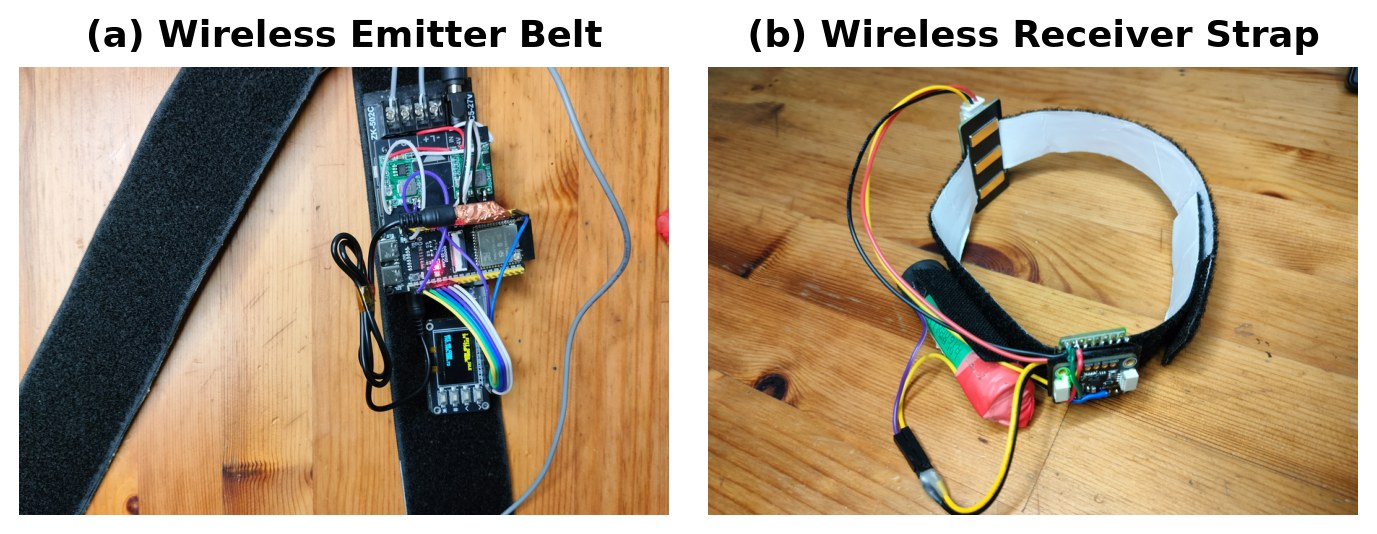
\includegraphics[width=0.90\columnwidth]{figures/fig0_hardware_prototype.jpg}
\caption{Untethered Microresonance prototype ($<\$100$ commodity BOM): (a) wireless active acoustic emitter belt and (b) dry wireless receiver strap operating through clothing with zero interconnecting cables.}
\label{fig:hw}
\end{figure}

\subsection{Wireless TSF-Locked Hardware and Embedded DSP}
Free-running MCU crystals drift by $10\text{--}20\text{ ppm}$ ($\sim 1800^\circ/\text{s}$ phase walk at $500\text{ Hz}$), destroying lock-in coherence within milliseconds. Microresonance eliminates this drift across two untethered ESP32-S3 nodes (Fig.~\ref{fig:hw}):
\begin{itemize}
    \item \textbf{Active Emitter Belt:} Queries hardware 802.11 Wi-Fi Beacon TSF (\texttt{esp\_wifi\_get\_tsf\_time}) before each I2S DMA buffer and computes analytical phase $\phi_i = 2\pi[((t_{\text{TSF}}\cdot 10^{-6} + i/f_s)f_0) \bmod 1]$ at $f_s = 44.1\text{ kHz}$ into an APLL-clocked PCM5102A DAC, ZK-502C Class-D amplifier, and coil-driven tactile exciter (DAEX32EP-4).
    \item \textbf{Dual-Core Isolated Receiver Strap:} Core~1 runs deterministic $4000\text{ Hz}$ SPI bursts from an ADXL355 (20-bit, $\sim 3.9\,\mu g/\text{LSB}$), capturing hardware \texttt{DRDY} in an IRAM ISR and back-dating the TSF stamp by the measured ISR-to-SPI lag. Core~0 independently polls a co-located LSM6DSOX IMU and analog sEMG channel, eliminating $3.3\text{ V}$ SAR-ADC rail cross-talk into the ADXL355.
    \item \textbf{Zero-Aggregation UDP Telemetry:} Each $30\text{ ms}$ frame ($120\times 3$ ADXL355, $30\times 6$ IMU, $120$ sEMG samples) fits in a single MTU-safe 1460-byte \texttt{RawSyncPacket} (\texttt{0x4D58}) tagged with \texttt{IP\_TOS = 0xE0} (WMM \texttt{AC\_VO}), disabling 802.11 A-MPDU aggregation ($5{,}135/5{,}136$ frames delivered, $99.98\%$).
\end{itemize}

\begin{figure*}[!t]
\centering
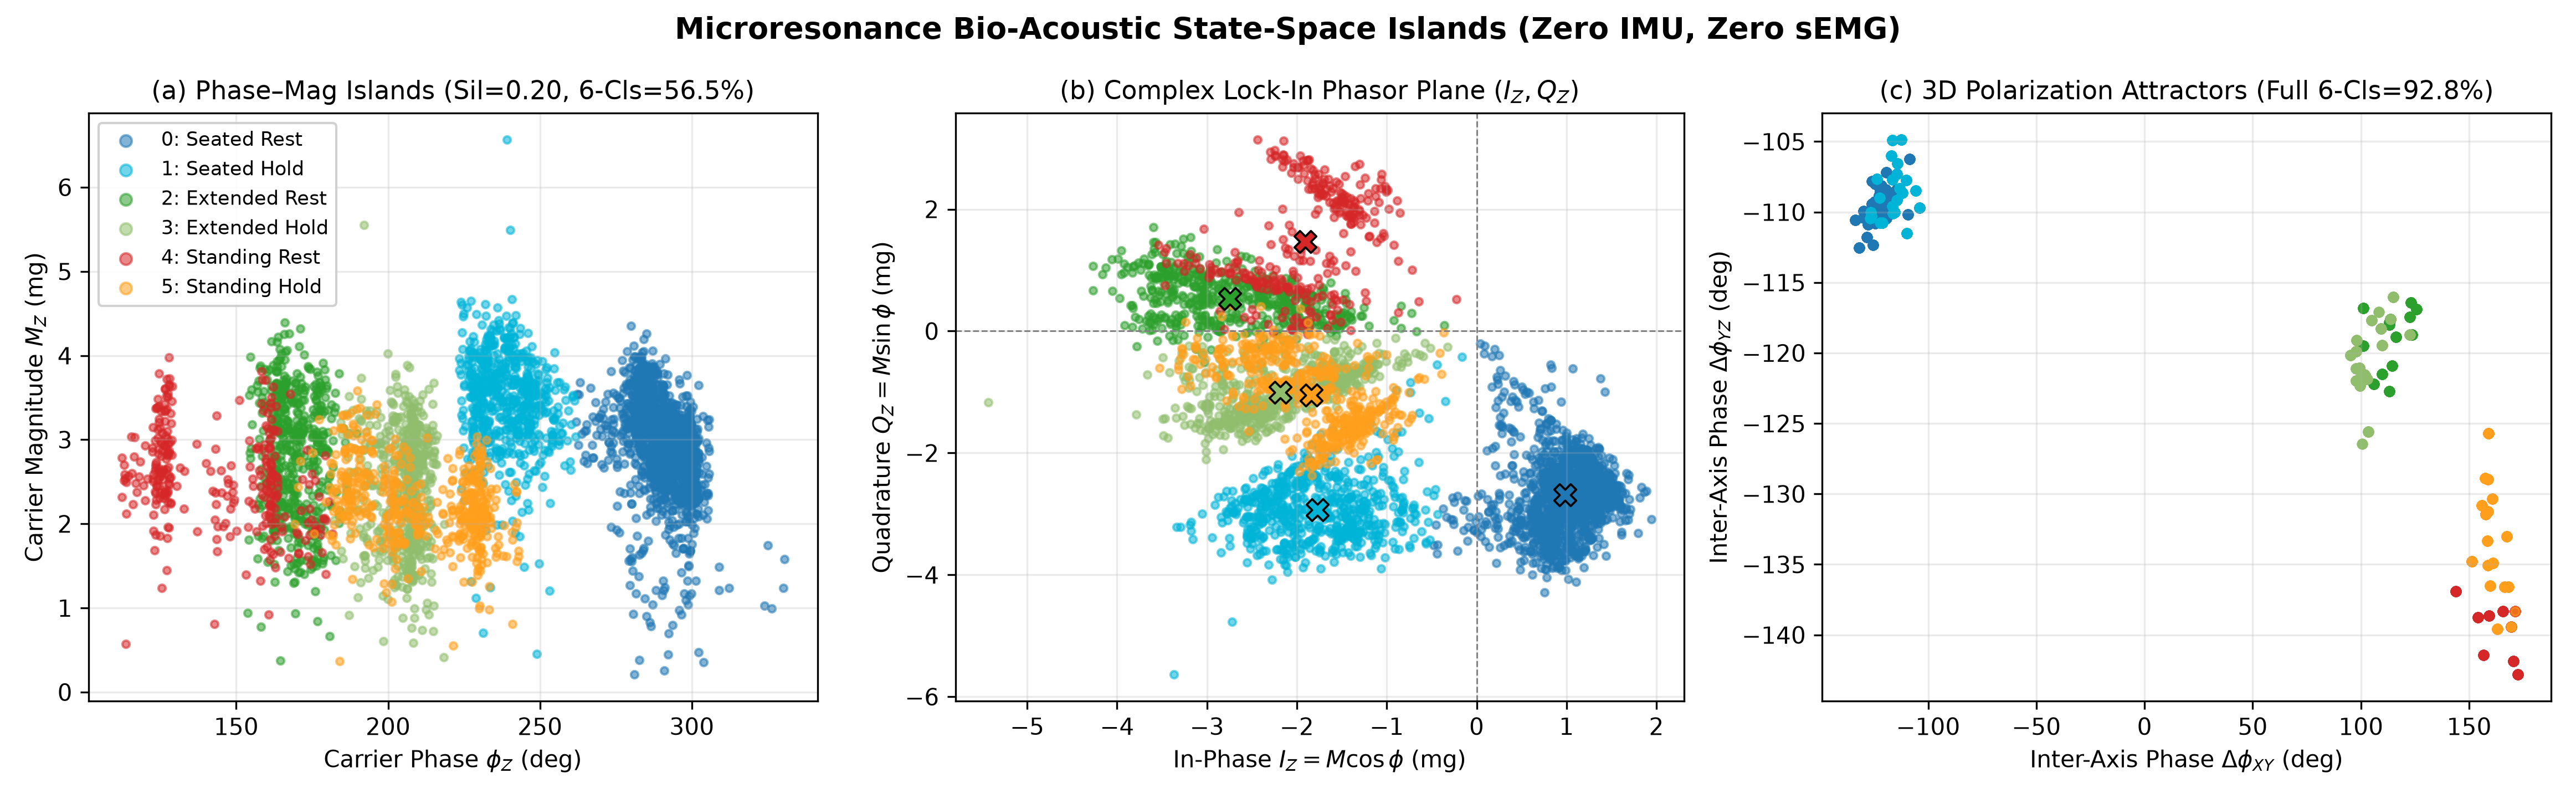
\includegraphics[height=1.24in]{figures/fig1_islands_state_space.png}
\caption{Bio-acoustic state-space islands across 6 biomechanical states (3 postures $\times$ \{rest, isometric hold\}, $N=1$) using only the $500\text{ Hz}$ ADXL355 lock-in signal (zero IMU, zero sEMG): (a) Phase--Magnitude islands ($56.5\%$), (b) Complex lock-in phasor plane $(I_Z, Q_Z)$, and (c) 3D polarization attractors $(\Delta\phi_{XY}, \Delta\phi_{YZ})$ lifting full 6-state holdout accuracy to $92.8\%$ (Silhouette $+0.46$).}
\label{fig:islands}
\end{figure*}

\subsection{TSF-Coherent Quadrature Lock-In Demodulation}
For each $30\text{ ms}$ window starting at $t_{\text{TSF}}$ with DC-removed samples $\tilde{x}_k$ ($k=0\dots N-1$, $\Delta t = 250\,\mu\text{s}$), the demodulator computes:
\begin{align}
I &= \sum_{k=0}^{N-1} \tilde{x}_k \cos\!\big(2\pi f_0 (t_{\text{TSF}}\cdot 10^{-6} + k\Delta t)\big), \\
Q &= \sum_{k=0}^{N-1} \tilde{x}_k \sin\!\big(2\pi f_0 (t_{\text{TSF}}\cdot 10^{-6} + k\Delta t)\big),
\end{align}
yielding magnitude $M = \frac{2}{N}\sqrt{I^2+Q^2}$ and demodulated phase lag $\phi = \operatorname{atan2}(Q,I) = -\arg H(\omega)$ (so a decrease $\Delta\phi < 0$ represents a positive phase lead $\Delta(\arg H) > 0$). Coherent 1~s vector integration across X, Y, Z yields inter-axis differential phases $\Delta\phi_{XY} = \phi_X - \phi_Y$ and $\Delta\phi_{YZ} = \phi_Y - \phi_Z$.

\section{Experimental Evaluation}

\subsection{Protocol and Non-Circular Spectral Validation}
We evaluated a single-subject ($N=1$) proof-of-concept session ($153.74\text{ s}$, $5{,}136$ frames at $33.41\text{ Hz}$, $f_0 = 500\text{ Hz}$, lumbar emitter belt to dry ankle strap over clothing, $\sim 0.9\text{ m}$ path) during voluntary whole-leg isometric co-contractions (coupled thigh and calf musculature along the waist-to-ankle chain, with the trunk kept neutral) across five regimes: (1) seated rest ($0\text{--}30\text{ s}$), (2) seated $5\text{ s}$ tension/relaxation cycles ($30\text{--}68\text{ s}$), (3) seated leg extension with $5\text{ s}$ cycles ($72\text{--}104\text{ s}$), (4) standing orthostatic load with voluntary holds ($111\text{--}135\text{ s}$), and (5) seated return ($140\text{--}153.7\text{ s}$).

During static rest ($5\text{--}25\text{ s}$), detrended phase noise was $3.01^\circ$ ($0.05\text{ rad}$, drift $-0.516^\circ/\text{s}$) with $99.9\%$ hard-lock despite $47.9\%$ peak-to-peak ($p_{95}\text{--}p_5$, $\text{CV}=15.6\%$) carrier-amplitude fluctuations from respiration and belt-coupling micro-variations ($\text{Corr}(M,\phi)=+0.075$), indicating low sensitivity of phase to passive amplitude drift. Exploiting the known $0.10\text{ Hz}$ fundamental ($10\text{ s}$ period) of the $5\text{ s}$ ON / $5\text{ s}$ OFF protocol, we computed non-circular protocol-band SNR ($0.07\text{--}0.13\text{ Hz}$ peak vs.\ $0.35\text{--}5.0\text{ Hz}$ noise floor) and fractional variance in the fundamental + 3rd harmonic ($0.10, 0.30\text{ Hz}$) across all five modalities (Table~\ref{tab:snr}, Fig.~\ref{fig:snr}).

\begin{table}[t]
\centering
\caption{Non-Circular Protocol-Frequency ($0.10\text{ Hz}$) SNR and Square-Wave Energy Concentration Across Modalities ($N=1$)}
\label{tab:snr}
\resizebox{\columnwidth}{!}{%
\begin{tabular}{lccc}
\toprule
\textbf{Modality} & \textbf{Seated} & \textbf{Leg Extended} & \textbf{Standing} \\
 & ($30\text{--}68\text{ s}$) & ($72\text{--}104\text{ s}$) & ($111\text{--}135\text{ s}$) \\
\midrule
\textbf{Acoustic Phase (500 Hz)} & \textbf{33.0 dB (82.3\%)} & \textbf{31.3 dB (73.3\%)} & \textbf{28.2 dB (39.0\%)} \\
Acoustic Mag (500 Hz) & 14.2 dB (5.9\%) & 23.2 dB (14.2\%) & 15.7 dB (10.4\%) \\
IMU Tilt (LSM6DSOX) & 20.6 dB (31.2\%) & 21.5 dB (33.7\%) & 16.9 dB (19.3\%) \\
sEMG (raw std) & 14.2 dB (6.5\%) & 5.4 dB (1.9\%) & 4.4 dB (1.8\%) \\
sEMG (high-pass diff) & 14.9 dB (6.6\%) & 4.6 dB (1.4\%) & 5.8 dB (1.7\%) \\
\bottomrule
\end{tabular}}
\end{table}

\subsection{Orthostatic Resilience and Bio-Acoustic State-Space Islands}
Unsupervised 1D 2-means clustering on detrended acoustic phase cleanly recovers the $5\text{ s}$ plateaus (seated step $45.1^\circ$, Cohen's $d = 5.51$; extended $36.0^\circ$, $d = 6.62$; standing $66.1^\circ$, $d = 3.57$), whereas sEMG collapses under leg extension ($d = 0.04$, AUC $= 0.51$) and standing load ($20.7\times$ baseline floor surge from $9.8$ to $203.1$, $d = 0.25$). Tilt excursions remain $<1^\circ$ ($0.94^\circ$ seated, $0.70^\circ$ standing; $r = -0.146, 0.319$), ruling out inclinometer artifacts. Consistent with impedance loading of the skeletal waveguide, isometric contractions shift phase from seated rest ($\sim 295^\circ \to 240^\circ$) and anti-correlate with magnitude ($r = -0.32$ to $-0.43$, corresponding to $+11\text{--}16\%$ transmission gain).

Fig.~\ref{fig:islands} shows that the six biomechanical states form discrete state-space attractors (``islands''). While 2D phase--magnitude alone reaches $56.5\%$ 6-state chronological holdout accuracy (Silhouette $+0.20$), combining $(\phi_Z, M_Z)$ with 3D inter-axis polarization $(\Delta\phi_{XY}, \Delta\phi_{YZ})$ resolves all six states at \textbf{92.8\% chronological holdout accuracy} (Silhouette $+0.46$, zero IMU, zero sEMG) vs.\ $28.9\%$ (Silhouette $-0.24$) for sEMG alone.

\subsection{IMU-Free Posture Orthogonalization, Self-Gating \& 3D Anisotropy}
Fig.~\ref{fig:ortho} and Table~\ref{tab:posture} show that $(\Delta\phi_{XY}, \Delta\phi_{YZ})$ stay stable during $5\text{ s}$ isometric holds while switching sharply across postures, achieving \textbf{100.0\% 3-posture holdout accuracy without an IMU} ($N=1$). Upon returning to seated rest ($142\text{--}153\text{ s}$), wrapped phase returns to $277.0^\circ$ (vs.\ $295.3^\circ$ initial) and $\Delta\phi_{YZ}$ returns to $-109.9^\circ$ (vs.\ $-110.1^\circ$ initial).

\begin{table}[t]
\centering
\caption{3D Acoustic Polarization Signature Across Postures (No IMU)}
\label{tab:posture}
\resizebox{\columnwidth}{!}{%
\begin{tabular}{lccc}
\toprule
\textbf{Posture Regime} & $\Delta\phi_{XY}$ (deg) & $\Delta\phi_{YZ}$ (deg) & $\Delta\phi_{XZ}$ (deg) \\
\midrule
Seated ($5\text{--}65\text{ s}$) & $-120.4 \pm 6.2$ & $-109.2 \pm 1.5$ & $+130.4 \pm 7.0$ \\
Leg Extended ($72\text{--}104\text{ s}$) & $+107.8 \pm 9.0$ & $-119.9 \pm 2.2$ & $-12.0 \pm 10.4$ \\
Standing ($111\text{--}135\text{ s}$) & $+160.9 \pm 6.5$ & $-135.2 \pm 4.4$ & $+25.6 \pm 6.3$ \\
\bottomrule
\end{tabular}}
\end{table}

\begin{figure*}[!t]
\centering
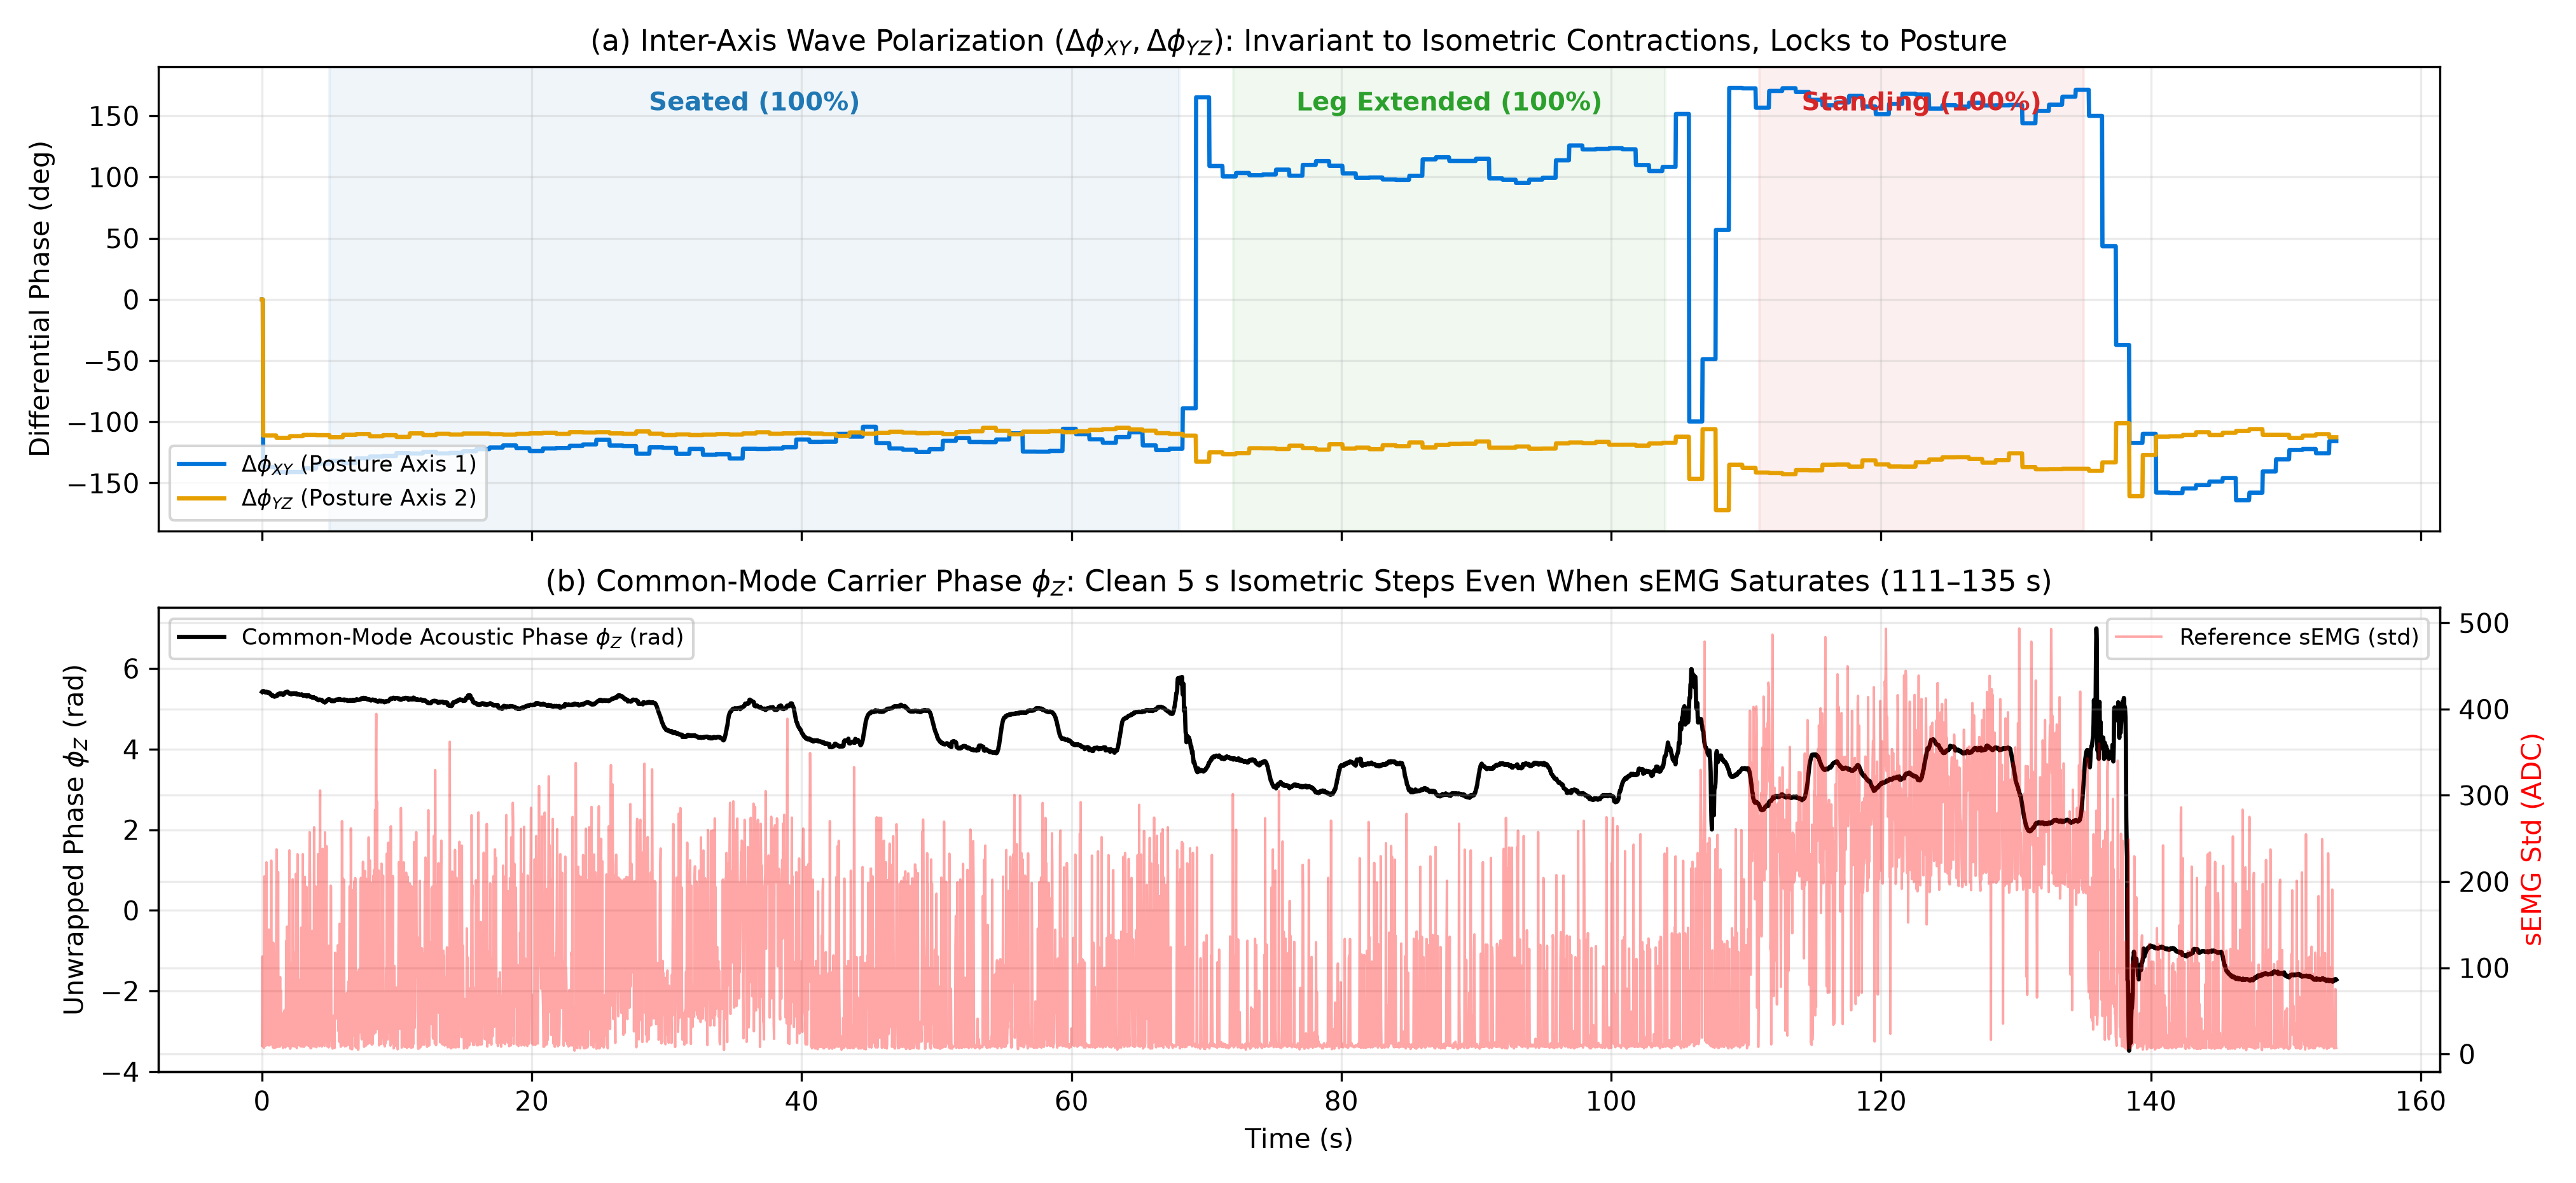
\includegraphics[height=1.00in]{figures/fig3_polarization_orthogonality.png}
\caption{Orthogonal decoupling of posture and motor intent ($N=1$): (a) Inter-axis polarization $(\Delta\phi_{XY}, \Delta\phi_{YZ})$ classifies all three postures at $100\%$ accuracy without IMU fusion; (b) Common-mode phase $\phi_Z$ resolves discrete $5\text{ s}$ isometric holds under standing orthostatic sEMG saturation ($111\text{--}135\text{ s}$).}
\label{fig:ortho}
\vspace{2pt}
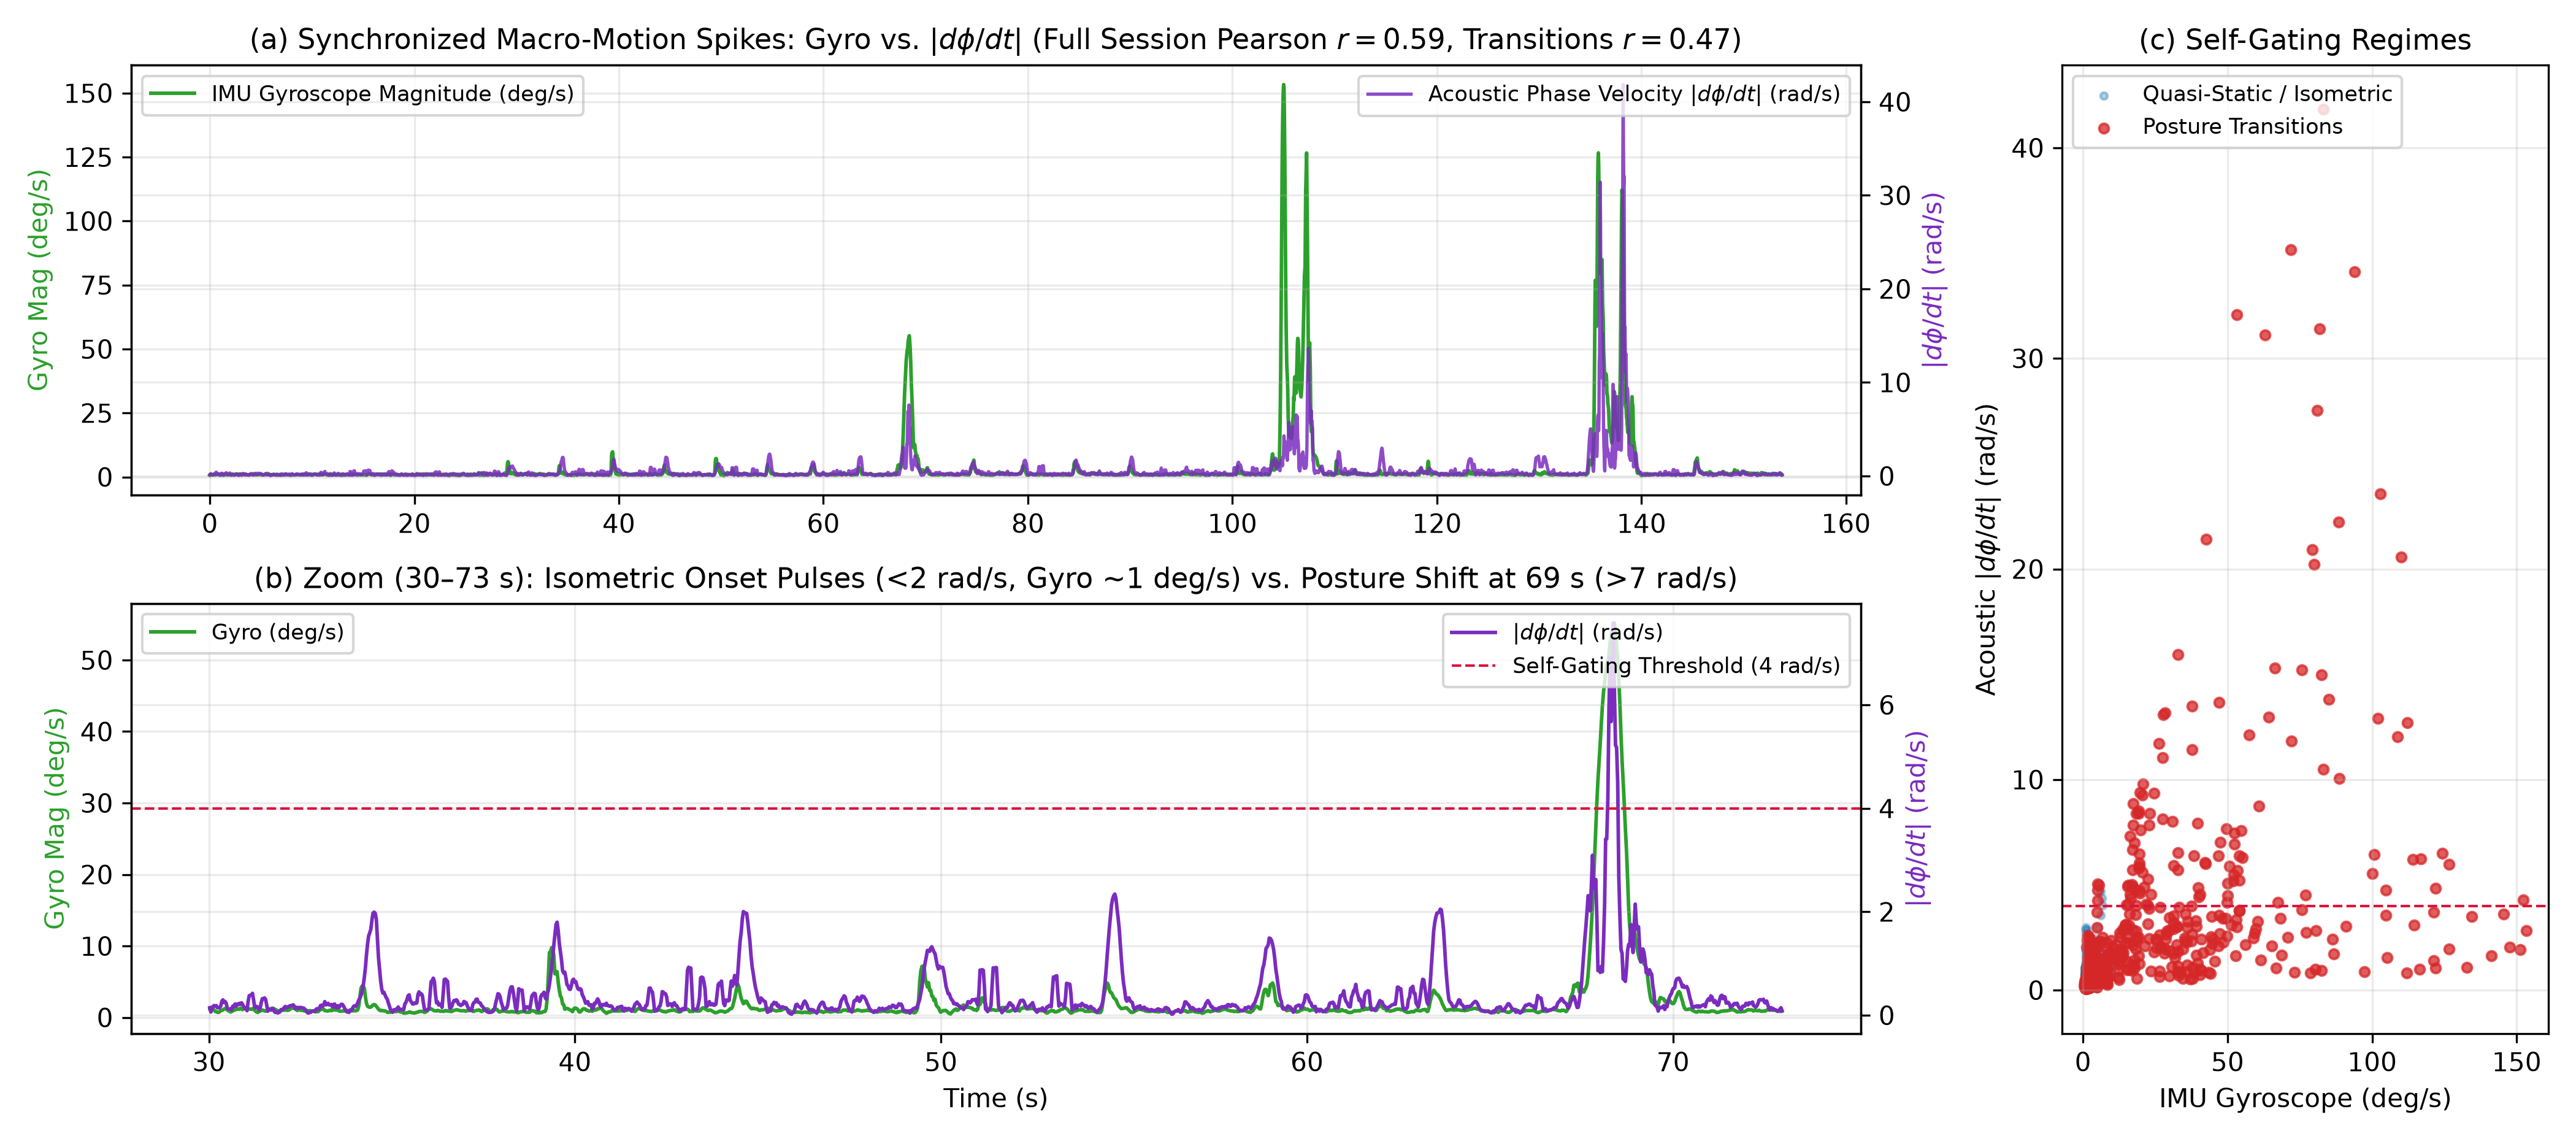
\includegraphics[height=1.00in]{figures/fig4_gyro_vs_phase_velocity.png}
\caption{Acoustic phase velocity $|d\phi/dt|$ vs.\ co-located IMU gyroscope: (a) Full-session synchronized macro-motion spikes ($r = 0.59$), (b) Zoom ($30\text{--}73\text{ s}$) separating isometric onset pulses ($\le 2.34\text{ rad/s}$) from the $69\text{ s}$ posture transition ($>7\text{ rad/s}$), and (c) Regime scatter showing $17.9\times$ separation for IMU-free self-gating at $4\text{ rad/s}$.}
\label{fig:gyro}
\end{figure*}

Acoustic phase velocity $|d\phi/dt|$ correlates strongly with the co-located LSM6DSOX gyroscope (Fig.~\ref{fig:gyro}; Pearson $r = 0.59$, Spearman $\rho = 0.45$). Peak $|d\phi/dt|$ during posture transitions ($69, 106, 137\text{ s}$) reaches $41.8\text{ rad/s}$, whereas static isometric onset/release pulses ($30\text{--}66\text{ s}$, median gyro $0.96^\circ/\text{s}$) remain $\le 2.34\text{ rad/s}$ - a \textbf{$17.9\times$ separation} enabling IMU-free motion self-gating at $|d\phi/dt| > 4\text{ rad/s}$.

\textbf{3-Axis Verification \& Orthostatic Anisotropy:} All three ADXL355 axes ($\phi_X, \phi_Y, \phi_Z$) independently achieve $30.7\text{--}30.8\text{ dB}$ mean protocol SNR ($80.5\text{--}81.9\%$ seated energy), ruling out single-axis artifacts, whereas the consumer LSM6DSOX $500\text{ Hz}$ channel exhibits static gravity leakage ($r = +0.96$ with $a_y$). On unique $1\text{ Hz}$ coherent updates ($n=156$), the drive-invariant ratio $M_Z/M_Y$ holds $1.26 \pm 0.02$ (seated rest), $1.28 \pm 0.04$ (seated isometric), and $1.30 \pm 0.07$ (extended), drops $>6\sigma$ to $1.02 \pm 0.03$ under standing load, and recovers to $1.22 \pm 0.07$ upon seated return.

\section{Comparison, Limitations \& Roadmap}
Table~\ref{tab:waves} contrasts Microresonance against WAVES~\cite{rohal2026waves}. Whereas WAVES targets slow resting stiffness over local soft tissue ($2.5\text{--}8.5\text{ cm}$), Microresonance exploits long-range skeletal-waveguide probing ($\sim 0.9\text{ m}$) for real-time ($30\text{ ms}$) dry through-clothing intent and posture decoding, targeting AR/VR wearables, bionic prosthetics, and exoskeletons backed by \texttt{WO/2026/229867}~\cite{fatkulin2026pct}.

\begin{table}[t]
\centering
\caption{Comparison Between WAVES (2026) and Microresonance}
\label{tab:waves}
\resizebox{\columnwidth}{!}{%
\begin{tabular}{lll}
\toprule
\textbf{Aspect} & \textbf{WAVES~\cite{rohal2026waves}} & \textbf{Microresonance (Ours)} \\
\midrule
Physical path & Local soft tissue ($2.5\text{--}8.5\text{ cm}$) & Skeletal waveguide ($\sim 0.9\text{ m}$) \\
Target task & Passive resting stiffness & Real-time intent + posture \\
Latency & $60\text{--}120\text{ s}$ ($33\text{--}98\%$ rej.) & $30\text{ ms}$ ($33.4\text{ Hz}$, $99.9\%$ lock) \\
Sync & Wired single-PCB array & Wireless 802.11 TSF ($<2\,\mu\text{s}$) \\
Sensing & Pulsed TDoA (3 IMUs) & Continuous I/Q lock-in (1 ADXL355) \\
Coupling & Bare-skin adhesive + stencil & Dry strap through clothing \\
\bottomrule
\end{tabular}}
\end{table}

\textbf{Limitations \& Falsifiable Controls:} This $N=1$ study lacks dynamometry, clinical wet-gel filtered sEMG, and quantitative strap-tension variation data. Moreover, over a $0.9\text{ m}$ waist-to-ankle path, two alternative mechanisms can contribute to $\Delta\phi$: (a) residual \textit{emitter-side lumbar coupling} (even with neutral seated/standing trunk posture minimizing voluntary core recruitment), and (b) \textit{joint compression} altering knee/hip articular contact. Ongoing work directly isolates these effects via: (i) a co-located reference accelerometer on the emitter belt to compute source-normalized $H = A_{\text{distal}}/A_{\text{ref}}$, (ii) multi-tone / stepped-frequency TSF lock-in spanning low-frequency tones (below tens-of-Hz tissue resonances $\omega_0$, where motion rejection is harder) up to $1000\text{ Hz}$ to test the predicted $\Delta|H|$ sign reversal across $\omega_0$, (iii) controlled strap-tension, over-bone vs.\ muscle-belly, off-path muscle, and passive-load tests, and (iv) $N \ge 10$ validation with a load cell and clinical sEMG.

\begin{thebibliography}{8}
\setlength{\itemsep}{1pt}
\bibitem{laput2016viband}
G. Laput, R. Xiao, and C. Harrison, ``ViBand: High-Fidelity Bio-Acoustic Sensing Using Commodity Smartwatch Accelerometers,'' in \textit{Proc.\ ACM UIST}, 2016, pp.\ 321--333.
\bibitem{akhlaghi2016smg}
N. Akhlaghi \textit{et al.}, ``Real-Time Classification of Hand Motions Using Ultrasound Imaging of Forearm Muscles,'' \textit{IEEE Trans.\ Biomed.\ Eng.}, vol.\ 63, no.\ 8, pp.\ 1687--1698, 2016.
\bibitem{gennisson2013elastography}
J.-L. Gennisson \textit{et al.}, ``Ultrasound elastography: Principles and techniques,'' \textit{Diagn.\ Interv.\ Imaging}, vol.\ 94, no.\ 5, pp.\ 487--495, 2013.
\bibitem{rohal2026waves}
S. Rohal, D. Y. Lee, and S. Pan, ``WAVES: Wearable Active Vibroacoustic Elasticity Sensing for Low-Cost and Non-Invasive Muscle Stiffness Monitoring,'' \textit{arXiv:2611.07087}, Nov.\ 4, 2026.
\bibitem{ieee80211}
\textit{IEEE Standard for Information Technology - Wireless LAN MAC and PHY Specifications}, IEEE Std 802.11, Timing Synchronization Function (TSF).
\bibitem{nigg2001tuning}
B. M. Nigg and J. M. Wakeling, ``Impact forces and muscle tuning: a new paradigm,'' \textit{Exerc.\ Sport Sci.\ Rev.}, vol.\ 29, no.\ 1, pp.\ 37--41, 2001.
\bibitem{wakeling2001leg}
J. M. Wakeling and B. M. Nigg, ``Modification of soft tissue vibrations in the leg by muscular activity,'' \textit{J.\ Appl.\ Physiol.}, vol.\ 90, no.\ 2, pp.\ 412--420, 2001.
\bibitem{fatkulin2026pct}
A. Fatkulin, ``System and Method for Active and Passive Vibrational Probing, Coherent Demodulation, Multi-Gate Semantic Tokenization, and Spatial Mapping of Biomechanical Transfer Functions,'' WIPO Pub.\ WO/2026/229867 (PCT/IB2026/054169), priority Apr.--May 2025, pub.\ Nov.\ 5, 2026.
\end{thebibliography}

\end{document}
